\chapter{Аналитический раздел}
В данном разделе проводится анализ предметной области, анализ подходов к синтезу изображений трёхмерного объекта, осуществляется описание сцены, трёхмерных объектов на сцене, проводится сравнительный анализ различных алгоритмов и обзор существующих методов.

\section{Формализация объектов сцены}
В компьютерной графике сцена является объектом, описывающим трёхмерное пространство и все объекты, находящиеся в данном трёхмерном пространстве.

В реализуемом программном обеспечении сцена содержит компоненты следующих типов:
\begin{itemize}
 \item источник света --- задаёт овещение сцены;
 \item трёхмерный объект --- трёхмерная модель, находящаяся на сцене;
 \item камера --- виртуальная камера, позволяющая просматривать трёхмерные объекты, находящиеся на сцене и делать их снимки.
\end{itemize}

\section{Анализ виртуальной камеры}
Виртуальная камера --- объект сцены трёхмерной виртуальной среды, эмулирующий камеру в трёхмерном пространстве сцены и позволяющий получать двумерный снимок (проекцию) сцены.

Проекция --- изображение трёхмерной фигуры на так называемой проекционной плоскости (экране) способом, представляющим собой геометрическую идеализацию оптических механизмов зрения, фотографии, камеры-обскуры.

Существует два основных вида проецирования:
\begin{itemize}
\item параллельная проекция;
\item перспективная проекция.
\end{itemize}

Параллельная проекция --- это проекция объекта в трехмерном пространстве на неподвижную плоскость, известную как плоскость проекции или плоскость изображения, где лучи, известные как линии обзора или проекционные линии, параллельны друг другу. 

Перспективная проекция --- это приблизительное представление, обычно на плоской поверхности, изображения таким, каким оно видится глазу.

Для поставленной задачи наилучшим решением будет использовать перспективную проекцию, поскольку она содержит больше информации о положении трёхмерного объекта в пространстве.

\section{Описание способа представления поверхности}
Трёхмерная модель в разрабатываемом программном обеспечении загружается из объектного файла, имеющего формат OBJ. Данный формат подразумевает сохранение модели в поверхностном виде с помощью полигональной сетки, поэтому для описания модели также используется поверхностный способ и полигональная сетка. Поскольку информация в файле содержит только описание точек и рёбер, то необходимо определить, каким образом будет представлена полигональная сетка. Существует четыре основных способа представления полигональной сетки:
\begin{itemize}
    \item Вершинное представление — полигональная сетка представляется как список, в котором для каждой вершине ставятся в соответствие вершины, с которыми она соединена рёбрами.
    \item Таблица углов — в данном случае вершины хранятся в предопределённой таблице.
    \item Список граней — объект представляется как множество граней и вершин.
    \item Список полигонов — объект представляется как множество элементарных поверхностей, формирующих поверхность модели. 
\end{itemize}

Для поставленной задачи наилучшим решением будет использование списка треугольных полигонов, поскольку треугольный полигон однозначно задаёт плоскость в трёхмерно пространстве и не требует дополнительных проходов по списку треугольных полигонов при отрисовке, что увеличивает скорость работы программы.

\section{Анализ алгоритмов удаления невидимых линий и поверхностей}
Алгоритм трассировки лучей --- при построении изображения луч посылается в заданном направлении для оценки приходящей оттуда световой энергии. Эта энергия определяется освещённостью первой поверхности, встретившейся на пути луча. Из каждого источника света выпускаются лучи во все стороны. При пересечении луча с поверхностью получаются отражённый и преломлённый лучи, а если моделировать диффузное освещение, то и пучок лучей, равномерно распространяющийся во все стороны. Данный метод имеет наивысшую степень реализма и вместе с этим высокую сложность реализации и затрат ресурсов при работе программы \cite{cgshish}.

Алгоритм Робертса --- Алгоритм Робертса представляет собой первое известное решение задачи об удалении невидимых линий. Это математически элегантный метод, работающий в объектном пространстве. Алгоритм прежде всего удаляет из каждого тела те ребра или грани, которые экранируются самим телом. Пусть F --- некоторая грань многогранника. Плоскость, несущая эту грань, разделяет пространство на два подпространства. Назовем положительным то из них, в которое смотрит внешняя нормаль к грани. Если точка наблюдения в положительном подпространстве, то грань лицевая, в противном случае  грань является нелицевой. Если многогранник выпуклый, то удаление всех нелицевых граней полностью решает задачу визуализации с удалением невидимых граней. Невыпуклые тела должны быть разбиты на выпуклые части. В этом алгоритме выпуклое многогранное тело с плоскими гранями должно представиться набором пересекающихся плоскостей \cite{cgshish}.

Алгоритм Варнака --- алгоритм Варнака является ещё одним примером алгоритма, основанного на разбиении картинной плоскости на части, для каждой из которых исходная задача может быть решена достаточно просто. Разобьём видимую часть картинной плоскости на 4 равные части. В случаях, когда часть полностью накрывается проекцией ближайшей грани и часть не накрывается проекцией ни одной грани, вопрос о закрашивании соответствующей части решается тривиально. В случае, когда ни одно из этих условий не выполнено, данная часть разбивается на 4 части, для каждой их которых проверяется выполнение этих условий, и так далее. Очевидно, что разбиение имеет смысл проводить до тех пор, пока размер части больше, чем размер пиксела \cite{cgshish_2}.

Алгоритм, использующий Z-буфер --- данный алгоритм является одним из простейших алгоритмов удаления невидимых поверхностей. Работает этот алгоритм в пространстве изображения. Идея Z-буфера является простым обобщением идеи о буфере кадра. Буфер кадра используется для запоминания атрибутов (интенсивности) каждого пиксела в пространстве изображения, Z-буфер --- это отдельный буфер глубины, используемый для запоминания координаты z или глубины каждого видимого пиксела в пространстве изображения. В процессе работы глубина или значение z каждого нового пиксела, который нужно занести в буфер кадра, сравнивается с глубиной того пиксела, который уже занесен в Z-буфер. Если это сравнение показывает, что новый пиксел расположен впереди пиксела, находящегося в буфере кадра, то новый пиксел заносится в этот буфер и, кроме того, производится корректировка Z-буфера новым значением z. Если же сравнение дает противоположный результат, то никаких действий не производится. По сути, алгоритм является поиском по х и у наибольшего значения функции z(х, у) \cite{cgshish}.

Для поставленной задачи наилучшим решением для реализации алгоритма удаления невидимых линий и поверхностей  будет использование алгоритма z-буфера, поскольку в данной задаче важна скорость построения изображения для динамической отрисовки трёхмерной сцены программы для просмотра моделей.

\section{Анализ методов закрашивания}

В компьютерной графике для расчета освещенности граней объектов применяется цветовая модель RGB. Интенсивность отраженного света точек объектов вычисляют отдельно для каждой их трех составляющих цветовых компонент, а затем объединяют в результирующую тройку цветов. При расчете освещенности граней применяют следующие типы освещения и отражения света от поверхностей: 
\begin{itemize}
\item рассеянное;
\item диффузное;
\item зеркальное.
\end{itemize}

Матовые поверхности обладают свойством диффузного отражения, т. е. равномерного по всем направлениям рассеивания света. Поэтому кажется, что поверхности имеют одинаковую яркость независимо от угла обзора. Для таких поверхностей справедлив закон косинусов Ламберта, устанавливающий соответствие между количеством отраженного света и косинусом угла $\theta$ между направлением на точечный источник света интенсивности $I_{p}$ и нормалью к поверхности. При этом количество отраженного света не зависит от положения наблюдателя. Освещенность рассеянным светом вычисляется по формуле \ref{light_dist}.
\begin{equation}\label{light_dist} 
I_{d} = I_{p} \cdot k_{d} \cdot cos \theta.
\end{equation}
Значение коэффициента диффузного отражения $k_{d}$ является константой в диапазоне (0, 1) и зависит от материала \cite{belcg}.

Закраска по Гуро — алгоритм закраски поверхности по Гуро позволяет устранить дискретность изменения интенсивности. Процесс закраски по методу Гуро осуществляется в четыре этапа:
\begin{enumerate}
\item вычисляются нормали ко всем полигонам;
\item определяются нормали в вершинах путем усреднения нормалей по всем полигональным граням, которым принадлежит вершина;
\item используя нормали в вершинах и применяя произвольный метод закраски, вычисляются значения интенсивности в вершинах;
\item каждый многоугольник закрашивается путем линейной интерполяции значений интенсивностей в вершинах сначала вдоль каждого ребра, а затем и между ребрами вдоль каждой сканирующей строки.
\end{enumerate}

Закраска по Фонгу — В методе закраски Фонга используется интерполяция вектора нормали к поверхности вдоль видимого интервала на сканирующей строке внутри многоугольника, а не интерполяция интенсивности. Интерполяция выполняется между начальной и конечной нормалями, которые сами тоже являются результатами интерполяции вдоль ребер многоугольника между нормалями в вершинах. Нормали в вершинах, в свою очередь, вычисляются так же, как в методе закраски, построенном на основе интерполяции интенсивности. В каждом пикселе вдоль сканирующей строки новое значение интенсивности вычисляется с помощью любой модели закраски. Заметные улучшения по сравнению с интерполяцией интенсивности наблюдаются в случае использования модели с учетом зеркального отражения, т. к. при этом более точно воспроизводятся световые блики. Однако даже если зеркальное отражение не используется, интерполяция векторов нормали приводит к более качественным результатам, чем интерполяция интенсивности, поскольку аппроксимация нормали в этом случае осуществляется в каждой точке \cite{belcg}.

Для поставленной задачи наилучшим решением будет метод простой диффузной закраски с использованием закона Ламберта, поскольку программа для просмотра моделей должна работать в режиме реального времени и не требуется рассчёт отражений и бликов при построении изображения модели.

\section{Описание получения изображения трёхмерного объекта}
Получение изображения трёхмерного объекта подразумевает преобразование математической пространственной модели в плоскую (растровую) картинку. Как структура данных, изображение на экране представляется матрицей точек, где каждая точка определена, по крайней мере, тремя числами: интенсивностью красного, синего и зелёного цвета. Таким образом, рендеринг преобразует трёхмерную векторную структуру данных в плоскую матрицу пикселей. 

Для того, чтобы построить двумерное изображение нам необходимо получить проекцию сцены относительно наблюдателя, находящегося в пространстве сцены. При этом, для того, чтобы преобразовать сцену в пространство камеры (наблюдателя), и при этом сохранить перспективу, необходимо координату каждой точки сцены умножить на матрицу перспективной проекции. Матрица проекции отображает заданный диапазон усеченной пирамиды в пространство отсечения, и при этом манипулирует w-компонентой каждой вершины таким образом, что чем дальше от наблюдателя находится вершина, тем больше становится это w-значение. После преобразования координат в пространство отсечения, все они попадают в диапазон от -w до w (вершины, находящиеся вне этого диапазона, отсекаются).

Пусть:
\begin{itemize}
\item $h$ - высота экрана;
\item $w$ - ширина экрана;
\item $\theta$ - угол обзора;
\item $Z_{far}$ - дальнаяя граница видимости;
\item $Z_{near}$ - ближняя граница видимости.
\end{itemize}

Тогда $M$ - матрица проекции, вычисляющаяся по формуле \ref{proj_mat}.

\begin{equation}\label{proj_mat}
\begin{bmatrix}
(\frac{h}{w})\cdot \frac{1}{tan(\frac{\theta}{2})} & 0 & 0 & 0\\
0 & \frac{1}{tan(\frac{\theta}{2})} & 0 & 0\\
0 & 0 & \frac{Z_{far}}{Z_{far} - Z_{near}} & 0\\
0 & 0 & \frac{-Z_{far} \cdot Z_{near}}{Z_{far} - Z_{near}} & 0\\
\end{bmatrix}
\end{equation}

После того, как сцена была преобразована в пространство камеры, происходит растрирование каждого треугольного полигона модели. Для пикселей этого полигона устанавливается цветовое значение с учётом цвета полигона и освещённости полигона, которая рассчитывается по закону Ламберта. После чего область на изображении, соответствующая полигону, закрашивается с учётом невидимых объектов, который производится с помощью алгоритма z-буффера.

Для того, чтобы получить снимок модели, сначала создаётся изображение модели. После чего создаётся файл формата JPEG, куда заносится полученная при создании изображения матрица пикселей. Затем снимок сохраняется в директории компьютера, указываемой пользователем при запросе на сохранение снимка.

\section{Анализ алгоритмов определения наиболее вероятного соответствия объекта, изображённого на двумерном снимке, с одним из объектов из списка тел}

Распознавание образов — это отнесение исходных данных к определённому классу с помощью выделения существенных признаков, характеризующих эти данные, из общей массы данных. 

Классическая постановка задачи распознавания образов: Дано множество объектов. Относительно них необходимо провести классификацию. Множество представлено подмножествами, которые называются классами. Заданы: информация о классах, описание всего множества и описание информации об объекте, принадлежность которого к определённому классу неизвестна. Требуется по имеющейся информации о классах и описании объекта установить к какому классу относится этот объект.

Существует несколько способов распознавания образов:
\begin{itemize}
\item Оптическое распознавание --- данный метод подразумевает перебор вида объекта под различными углами, масштабами, смещениями. Тот образ, который менее всего отличается от разпознаваемого, выбирается в качестве результата распознания.
\item Исследование контура объекта --- данный способ подразнайти контур объекта и исследовать его свойства (связность, наличие углов и т.д.).
\item Использование исскуственных нейронных сетей ---  данный метод требует либо большого количества примеров задачи распознавания (с правильными ответами), либо специальной структуры нейронной сети, учитывающей специфику данной задачи.
\end{itemize}

Для данной задачи наилучшим решением будет использование исскуственных нейронных сетей, так как с помощью реализуемой программы для просмотра модели возможно генерировать примеры задачи распознавания в неограниченном количестве для каждого объекта. Помимо этого нейросети позволяют легко расширять количество классов, для этого достаточно дообучить эту нейросеть на изображениях, полученных с помощью программы для просмотра моделей для нового объекта.

Нейронная сеть --- математическая модель, а также её программное или аппаратное воплощение, построенная по принципу организации и функционирования биологических нейронных сетей --- сетей нервных клеток живого организма \cite{nn}.

\begin{figure}[H]
	\center{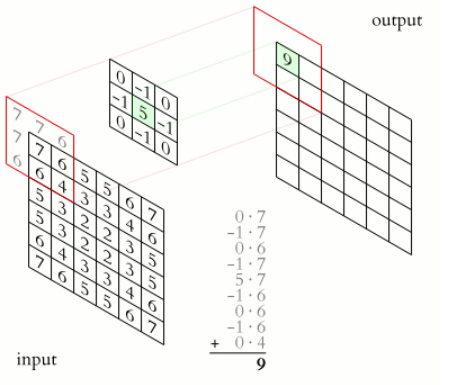
\includegraphics[scale=0.6]{conv_explain}}
	\caption{Схема свёрточной нейросети}
\end{figure}

Свёрточная нейросеть --- специальная архитектура искусственных нейронных сетей  нацеленная на эффективное распознавание образов. Данная архитектура использует некоторые особенности зрительной коры, в которой существуют простые клетки, реагирующие на прямые линии под разными углами, и сложные клетки, реакция которых связана с активацией определённого набора простых клеток. Таким образом, идея свёрточных нейронных сетей заключается в чередовании свёрточных слоёв и слоёв подвыборки. Структура сети — однонаправленная, многослойная. Для обучения используются стандартные методы, чаще всего метод обратного распространения ошибки. Основное отличие от многослойного перцептрона является наличие операции свёртки, суть которой заключается в том, что каждый фрагмент изображения умножается на матрицу свёртки поэлементно, а результат суммируется и записывается в аналогичную позицию выходного изображения. Работа свёрточной нейронной сети обычно интерпретируется как переход от конкретных особенностей изображения к более абстрактным деталям, и далее к ещё более абстрактным деталям вплоть до выделения понятий высокого уровня. При этом сеть самонастраивается и вырабатывает сама необходимую иерархию абстрактных признаков, фильтруя маловажные детали и выделяя существенное \cite{cnn}.

Для данной задачи наилучшим решением будет использование свёрточной нейронной сети, поскольку свёрточные нейронные сети, позволяют извлекать абстрактные признаки из изображений. Затем эти признаки используются моделью машинного обучения для определения вероятности соответствия входных данных определённому значению выхода нейросети.

\section{Описание трёхмерных преобразований}
Все трёхмерные преобразования являются результатом применения серии элементарных операций преобразования к какому-либо трёхмерному объекту. Данные элементарные преобразования включают в себя перемещение, мастабирование и поворот.

Рассмотрим операцию перемещения. Пусть координаты некоторой точки в трёхмерном пространстве задаются вектором $\overrightarrow{p} = \{p_{x}, p_{y}, p_{z}\}$, а вектор перемещения задаётся вектором $\overrightarrow{d} = \{d_{x}, d_{y}, d_{z}\}$, тогда координаты перемещённой точки в пространстве задаются вектором $\overrightarrow{p'}$, который вычисляется по формуле \ref{move}.

\begin{equation}\label{move} 
\overrightarrow{p'} = 
\begin{cases}
p'_{x} = p_{x} + d_{x}\\
p'_{y} = p_{y} + d_{y}\\
p'_{z} = p_{z} + d_{z}\\
\end{cases}
\end{equation}

Операция перемещения в матричном виде вычисляется по формуле \ref{move_mat}.

\begin{equation}\label{move_mat} 
\overrightarrow{p'} = 
\begin{bmatrix}
p_{x} & p_{y} & p_{z} & 0\\
\end{bmatrix}
\times
\begin{bmatrix}
1 & 0 & 0 & 0\\
0 & 1 & 0 & 0\\
0 & 0 & 1 & 0\\
d_{x} & d_{y} & d_{z} & 1\\
\end{bmatrix}
\end{equation}

Рассмотрим операцию мастабирования. Данная операция происходит относительно точки, называемой центром масштабирования. Пусть в этом случае центр масштабирования - начало координат, координаты некоторой точки в трёхмерном пространстве задаются вектором $\overrightarrow{p} = \{p_{x}, p_{y}, p_{z}\}$, а вектор коэффициентов масштабирования точки задаётся вектором $\overrightarrow{s} = \{s_{x}, s_{y}, s_{z}\}$, тогда координаты масштабированной относительно центра координат точки в пространстве задаются вектором $\overrightarrow{p'}$, который вычисляется по формуле \ref{scale}.

\begin{equation}\label{scale} 
\overrightarrow{p'} = 
\begin{cases}
p'_{x} = p_{x} \cdot s_{x}\\
p'_{y} = p_{y} \cdot s_{y}\\
p'_{z} = p_{z} \cdot s_{z}\\
\end{cases}
\end{equation}

Операция масштабирования в матричном виде вычисляется по формуле  \ref{scale_mat}.

\begin{equation}\label{scale_mat} 
\overrightarrow{p'} = 
\begin{bmatrix}
p_{x} & p_{y} & p_{z} & 0\\
\end{bmatrix}
\times
\begin{bmatrix}
s_{x} & 0 & 0 & 0\\
0 & s_{y} & 0 & 0\\
0 & 0 & s_{z} & 0\\
0 & 0 & 0 & 1\\
\end{bmatrix}
\end{equation}

Рассмотрим операцию поворота. Данная операция происходит относительно оси, называемой осью вращения. Рассмотрим вращение относительно осей $OX, OY, OZ$. Пусть координаты некоторой точки в трёхмерном пространстве задаются вектором $\overrightarrow{p} = \{p_{x}, p_{y}, p_{z}\}$, а угол поворота относительно оси равен $phi$.
Тогда координаты повернутой относительно осей $OX, OY, OZ$ точки в пространстве задаются векторами $\overrightarrow{p'_{OX}}, \overrightarrow{p'_{OY}}, \overrightarrow{p'_{OZ}}$, которые соответственно вычисляются по формулам \ref{rot_OX}, \ref{rot_OY}, \ref{rot_OZ}.

\begin{equation}\label{rot_OX} 
\overrightarrow{p'_{OX}} = 
\begin{cases}
p'_{x} = p_{x}\\
p'_{y} = p_{y} \cdot cos \phi + p_{z} \cdot sin \phi\\
p'_{z} = -p_{y} \cdot sin \phi + p_{z} \cdot cos \phi\\
\end{cases}
\end{equation}

\begin{equation}\label{rot_OY} 
\overrightarrow{p'_{OY}} = 
\begin{cases}
p'_{x} = p_{x} \cdot cos \phi - p_{z} \cdot sin \phi\\
p'_{y} = p_{y}\\
p'_{z} = p_{x} \cdot sin \phi + p_{z} \cdot cos \phi\\
\end{cases}
\end{equation}

\begin{equation}\label{rot_OZ} 
\overrightarrow{p'_{OZ}} = 
\begin{cases}
p'_{x} = p_{x} \cdot cos \phi + p_{y} \cdot sin \phi\\
p'_{y} = -p_{x} \cdot sin \phi + p_{z} \cdot cos \phi\\
p'_{z} = p_{z}\\
\end{cases}
\end{equation}

Операции поворота вокруг осей $OX, OY, OZ$ в матричном виде вычисляются по формулам \ref{rot_OX_mat},  \ref{rot_OY_mat},  \ref{rot_OZ_mat}.

\begin{equation}\label{rot_OX_mat} 
\overrightarrow{p'_{OX}} = 
\begin{bmatrix}
p_{x} & p_{y} & p_{z} & 0\\
\end{bmatrix}
\times
\begin{bmatrix}
1 & 0 & 0 & 0\\
0 & cos \phi & -sin \phi & 0\\
0 & sin \phi & cos \phi & 0\\
0 & 0 & 0 & 1\\
\end{bmatrix}
\end{equation}

\begin{equation}\label{rot_OY_mat} 
\overrightarrow{p'_{OY}} = 
\begin{bmatrix}
p_{x} & p_{y} & p_{z} & 0\\
\end{bmatrix}
\times
\begin{bmatrix}
cos \phi & 0 & sin \phi & 0\\
0 & 0 & 0 & 0\\
-sin \phi & 0 & cos \phi & 0\\
0 & 0 & 0 & 1\\
\end{bmatrix}
\end{equation}

\begin{equation}\label{rot_OZ_mat} 
\overrightarrow{p'_{OZ}} = 
\begin{bmatrix}
p_{x} & p_{y} & p_{z} & 0\\
\end{bmatrix}
\times
\begin{bmatrix}
cos \phi & -sin \phi & 0 & 0\\
sin \phi & cos \phi & 0 & 0\\
0 & 0 & 1 & 0\\
0 & 0 & 0 & 1\\
\end{bmatrix}
\end{equation}

\section{Описание требований к разрабатываемому программному обеспечению}
\subsection{Описание входных и выходных данных}
Входные и выходные данные делятся на две категории. Первая --- входные и выходные данные программы для просмотра модели, вторая --- входные и выходные данные алгоритма распознания трёхмерного объекта.

Входные данные программы для просмотра модели включают в себя параметры объектов сцены, вводимые пользователем при помощи интерфейса, адрес файла, содержащего трёхмерный объект, который необходимо загрузить в пространство сцены.

Выходные данные программы для просмотра модели включают в себя параметры объектов сцены, отображающиеся при их изменении, адрес файла, в который сохранён двумерный снимок сцены, адрес файла, в который сохранён трёхмерный объект, находящийся на сцене.

Входные данные алгоритма определения наиболее вероятного соответствия объекта, изображённого на двумерном снимке, с одним из объектов из списка тел включают в себя изображение, на котором изображён трёхмерный объект.

Выходные данные алгоритма определения наиболее вероятного соответствия объекта, изображённого на двумерном снимке, с одним из объектов из списка тел включают в себя трёхмерный объект, который был распознанс поданного на вход двумерного изображения.

\subsection{Описание функциональных требований к программному обеспечению}
Разрабатываемое ПО должно предоставлять следующий функционал:
\begin{itemize}
\item загрузка полигональных трёхмерных объектов из файлов;
\item загрузка трёхмерных объектов на сцену из заготовленного набора примитивов;
\item произведение простейших трансформаций (перемещение, масштабирование, вращение) над загруженным на сцену объектом;
\item навигация по сцене с помощью перемещения и поворота виртуальной камеры;
\item просмотр и изменение свойств объектов в сцене;
\item сохранение текущего изображения сцены в файл на диске;
\item сохранение просматриваемого трёхмерного объекта в файл;
\item определение наиболее вероятного соответствия объекта, изображённого на двумерном снимке, с одним из объектов из списка тел.
\end{itemize}

\section{Вывод из аналитического раздела}
В результате проведённого анализа были рассмотрены алгоритмы и методы, позволяющие решить задачу создания программного обеспечения, способного выводить на экран изображение трёхмерного объекта.  Были формализованы объекты сцены, включающие в себя источник света, трёхмерный объект и камеру. Для реализации виртуальной камеры была выбрана перспективная проекция. Для реализации представления поверхности трёхмерной модели был выбран поверхностный способ описания модели, представленный как полигональная сетка, задающаяся списком треугольных полигонов. Для реализации алгоритма удаления невидимых линий и поверхностей был выбран алгоритм z-буфера. Для реализации метода закрашивния был выбран метод простой диффузной закраски с использованием закона Ламберта. Для реализации алгоритма, позволяющего определять объект из списка объектов, изображённого на изображении, с одним из объектов из списка тел данной задачи наиболее подходит свёрточная нейронная сеть. Были описаны трёхмерные преобразования и преобразования сцены в пространство виртуальной камеры. Были описаны требования к разрабатываемому приложению.